\documentclass[11pt]{article}
\usepackage[margin=0.75in]{geometry}
\usepackage{amsmath,amssymb,tikz}
\usetikzlibrary{arrows.meta,positioning,calc}
\definecolor{resultblue}{RGB}{231,240,249}
\definecolor{modelgray}{RGB}{245,245,245}
\pagestyle{plain}
\setlength{\parindent}{0pt}
\hyphenpenalty=10000\exhyphenpenalty=10000
\tikzset{box/.style={draw,rounded corners=2pt,align=center,font=\small,text width=5cm,minimum height=1.2cm,inner sep=7pt},model/.style={box,fill=modelgray},result/.style={box,fill=resultblue},edge/.style={-{Latex[length=2mm]},thick}}
\begin{document}
\section*{A Testable Theory of Atomic Features}
\subsection*{Rigidity and generic dimension bounds}
An arrow means that a definition or result supplies a mathematical input.
The diagram shows paper-level statements; proof implementation details are
omitted. Result numbers follow the September 25 manuscript.

\begin{center}
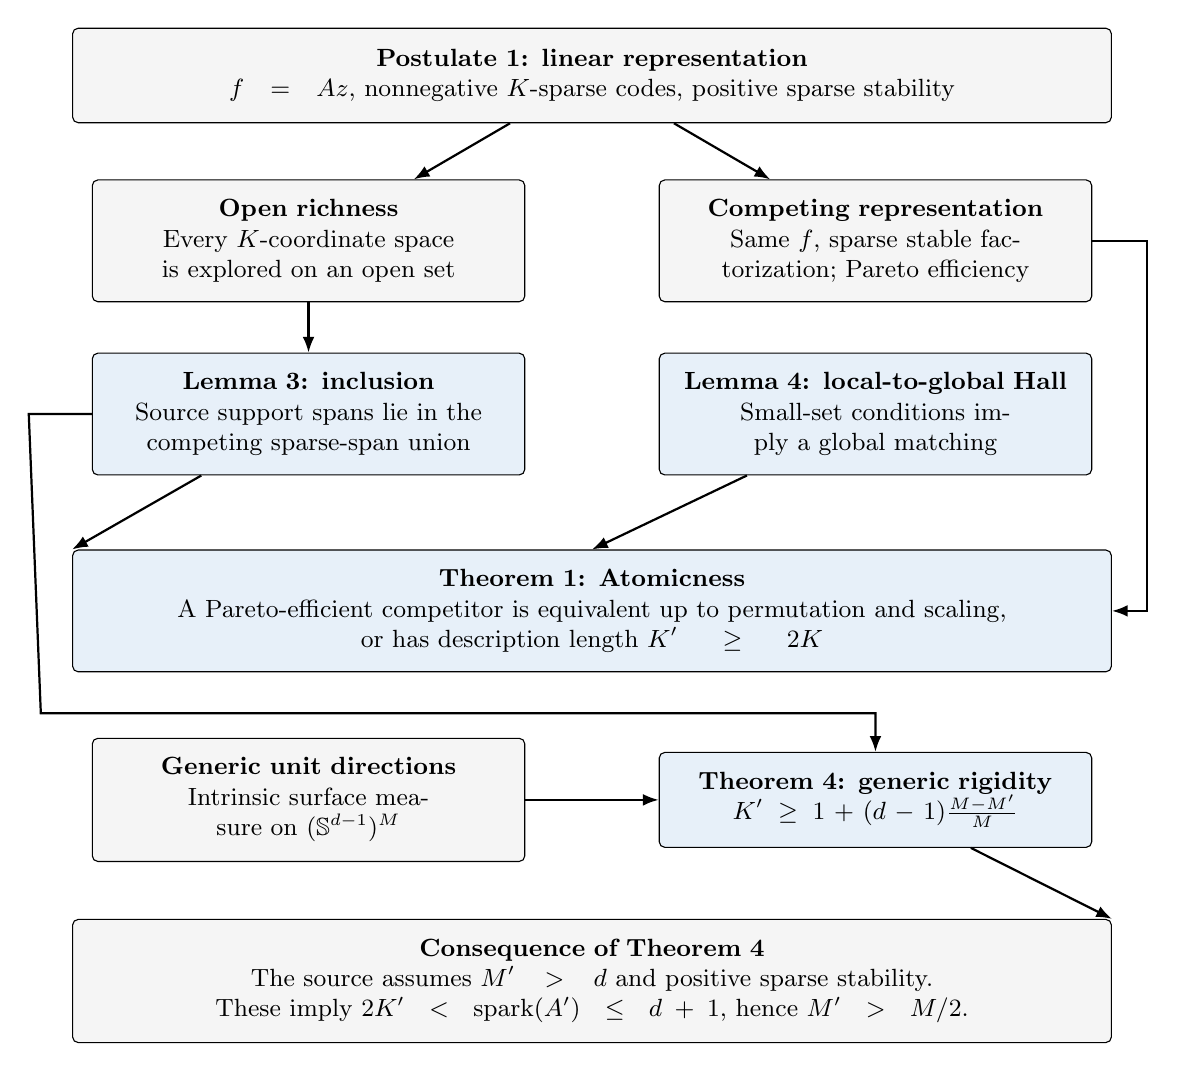
\begin{tikzpicture}
\node[model,text width=12.7cm] (atomic) at (0,0)
{\textbf{Postulate 1: linear representation}\\ $f=Az$, nonnegative $K$-sparse codes, positive sparse stability};
\node[model] (rich) at (-3.6,-2.1)
{\textbf{Open richness}\\Every $K$-coordinate space is explored on an open set};
\node[model] (compete) at (3.6,-2.1)
{\textbf{Competing representation}\\Same $f$, sparse stable factorization; Pareto efficiency};
\node[result] (inclusion) at (-3.6,-4.3)
{\textbf{Lemma 3: inclusion}\\Source support spans lie in the competing sparse-span union};
\node[result] (hall) at (3.6,-4.3)
{\textbf{Lemma 4: local-to-global Hall}\\Small-set conditions imply a global matching};
\node[result,text width=12.7cm] (rigid) at (0,-6.8)
{\textbf{Theorem 1: Atomicness}\\A Pareto-efficient competitor is equivalent up to permutation and scaling,\\or has description length $K'\ge2K$};
\node[model] (genericlaw) at (-3.6,-9.2)
{\textbf{Generic unit directions}\\Intrinsic surface measure on $(\mathbb S^{d-1})^M$};
\node[result] (generic) at (3.6,-9.2)
{\textbf{Theorem 4: generic rigidity}\\$K'\ge1+(d-1)\frac{M-M'}M$};
\node[model,text width=12.7cm] (half) at (0,-11.5)
{\textbf{Consequence of Theorem 4}\\The source assumes $M'>d$ and positive sparse stability.\\These imply $2K'<\operatorname{spark}(A')\le d+1$, hence $M'>M/2$.};
\draw[edge] (atomic)--(rich);
\draw[edge] (atomic)--(compete);
\draw[edge] (rich)--(inclusion);
\draw[edge] (compete.east)--++(0.7,0)|-(rigid.east);
\draw[edge] (inclusion)--(rigid.north west);
\draw[edge] (hall)--(rigid.north);
\draw[edge] (genericlaw)--(generic);
\draw[edge] (inclusion.west)--++(-0.8,0)--(-7.0,-8.1)--(3.6,-8.1)--(generic.north);
\draw[edge] (generic)--(half.north east);
\end{tikzpicture}
\end{center}
Generic rigidity quantifies over overcomplete competitors, as stated in the
source. Atomicness uses its own stated competing-dictionary class.

\clearpage
\section*{Recovery and its predictions}
All recovery statements use normalized source and learned columns, positive
sparse stability, nonnegative sparse codes, and a constant-factor bound on the
actual population reconstruction loss. Targets have positive prevalence.

\begin{center}
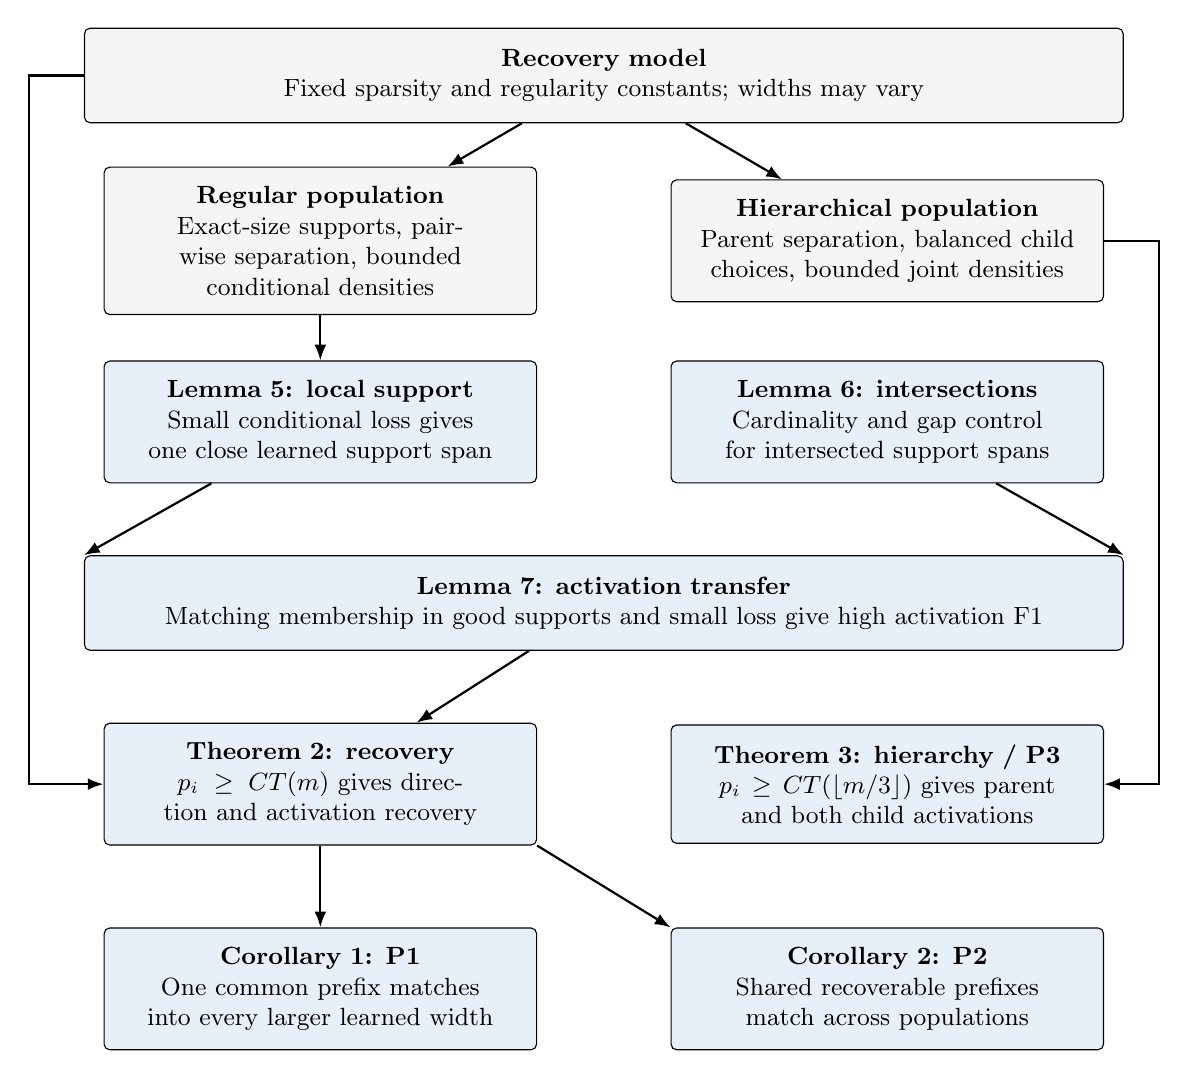
\begin{tikzpicture}
\node[model,text width=12.7cm] (base) at (0,0)
{\textbf{Recovery model}\\Fixed sparsity and regularity constants; widths may vary};
\node[model] (regular) at (-3.6,-2.1)
{\textbf{Regular population}\\Exact-size supports, pairwise separation, bounded conditional densities};
\node[model] (hierlaw) at (3.6,-2.1)
{\textbf{Hierarchical population}\\Parent separation, balanced child choices, bounded joint densities};
\node[result] (local) at (-3.6,-4.4)
{\textbf{Lemma 5: local support}\\Small conditional loss gives one close learned support span};
\node[result] (intersection) at (3.6,-4.4)
{\textbf{Lemma 6: intersections}\\Cardinality and gap control for intersected support spans};
\node[result,text width=12.7cm] (activation) at (0,-6.7)
{\textbf{Lemma 7: activation transfer}\\Matching membership in good supports and small loss give high activation F1};
\node[result] (recover) at (-3.6,-9)
{\textbf{Theorem 2: recovery}\\$p_i\ge C T(m)$ gives direction and activation recovery};
\node[result] (hier) at (3.6,-9)
{\textbf{Theorem 3: hierarchy / P3}\\$p_i\ge C T(\lfloor m/3\rfloor)$ gives parent and both child activations};
\node[result] (p1) at (-3.6,-11.6)
{\textbf{Corollary 1: P1}\\One common prefix matches into every larger learned width};
\node[result] (p2) at (3.6,-11.6)
{\textbf{Corollary 2: P2}\\Shared recoverable prefixes match across populations};
\draw[edge] (base)--(regular);
\draw[edge] (base)--(hierlaw);
\draw[edge] (regular)--(local);
\draw[edge] (local)--(activation.north west);
\draw[edge] (intersection)--(activation.north east);
\draw[edge] (activation)--(recover);
\draw[edge] (hierlaw.east)--++(0.7,0)|-(hier.east);
\draw[edge] (base.west)--++(-0.7,0)|-(recover.west);
\draw[edge] (recover)--(p1);
\draw[edge] (recover.south east)--(p2.north west);
\end{tikzpicture}
\end{center}
$T$ is the discarded prevalence tail (the parent tail for hierarchy).
No Zipf law or orthogonality is assumed. Hierarchy guarantees activation
recovery; it does not assert ordinary direction recovery of every child.
The support-pattern proof of Theorem 3 is described in the mathematical notes.
\end{document}
